\chapter{Context and Related Work}
\label{cha:related_work}
\minitoc

\section{Global Warming and ICT Role}
Global warming is one of the most critical environmental issues of our day \cite{houghton2005global}. Global warming is the effect of human activities on the climate, mainly the burning of fossil fuels (coal, oil, and gas) and large-scale deforestation \cite{houghton2005global}. Both activities have grown immensely since the industrial revolution. The burning of fossil fuels process results in greenhouse gas emissions \cite{olabi2022renewable}. Today, fossil fuels are one of the world's main sources of energy production, helping to emit more and more GHG \cite{olabi2022renewable}. GHG stays in the atmosphere creating a layer as a blanket over the planet's surface. Without this blanket, the Earth can balance the radiation energy from the sun and the thermal radiation from the Earth to space \cite{houghton2005global}. However, this human-generated blanket imposes a barrier to the thermal radiation from the Earth, letting it into the atmosphere and heating the planet, working as a greenhouse. All this process works as a greenhouse which is the reason for the name greenhouse gas \cite{houghton2005global}.

This situation brings us to United Nations Climate Change Conference (COP21) in Paris, France, on 12 December 2015. At this conference, 196 signed the Paris Agreement aiming to \cite{nations_paris_nodate}:
\begin{enumerate}
    \item Reduce global greenhouse gas emissions substantially, limiting the global temperature increase in this century to 2\degree C while pursuing measures to limit the growth even further to 1.5\degree C;
    \item Review countries’ commitments every five years (through the Nationally Determined Contribution, or NDC);
    \item Provide financing to developing countries to mitigate climate change, strengthen resilience, and enhance their abilities to adapt to climate impacts. 
\end{enumerate}

These are ambitious but necessary objectives. Since then, countries and organizations have proposed several actions and pledges. However, a recent report indicates that the actual world's effort is not enough \cite{tracker2022projections}. Figure \ref{fig:ghg_cat} shows GHG emission and temperature estimations. We could see that there is a small reduction in emissions increase tendency. Nevertheless, this figure estimates that real-world actions based on current policies will lead to an increase of somewhere between 2.6 and 2.9\degree C by 2100. This estimation is well above the 1.5\degree C pursued by the Paris Agreement. Considering the targets proposed by the countries through NDC, the temperature will be around 2.4\degree C. In a scenario based on NDC targets and submitted and binding long-term targets, the prediction is a temperature of 2\degree C by 2100, the limit proposed by the Paris Agreement. The report forecasts an optimistic scenario analyzing the effect of net zero emissions targets of about 140 countries that are adopted or under discussion. Even in this optimistic scenario, the estimated temperature would be 1.8\degree C. The situation tends to be even worst with the gold rush for gas \cite{tracker2022massive}. The report indicates that in 2022 we arrived at 1.2\degree C warming \cite{tracker2022projections}.

\begin{figure}[!htb]
    \centering
    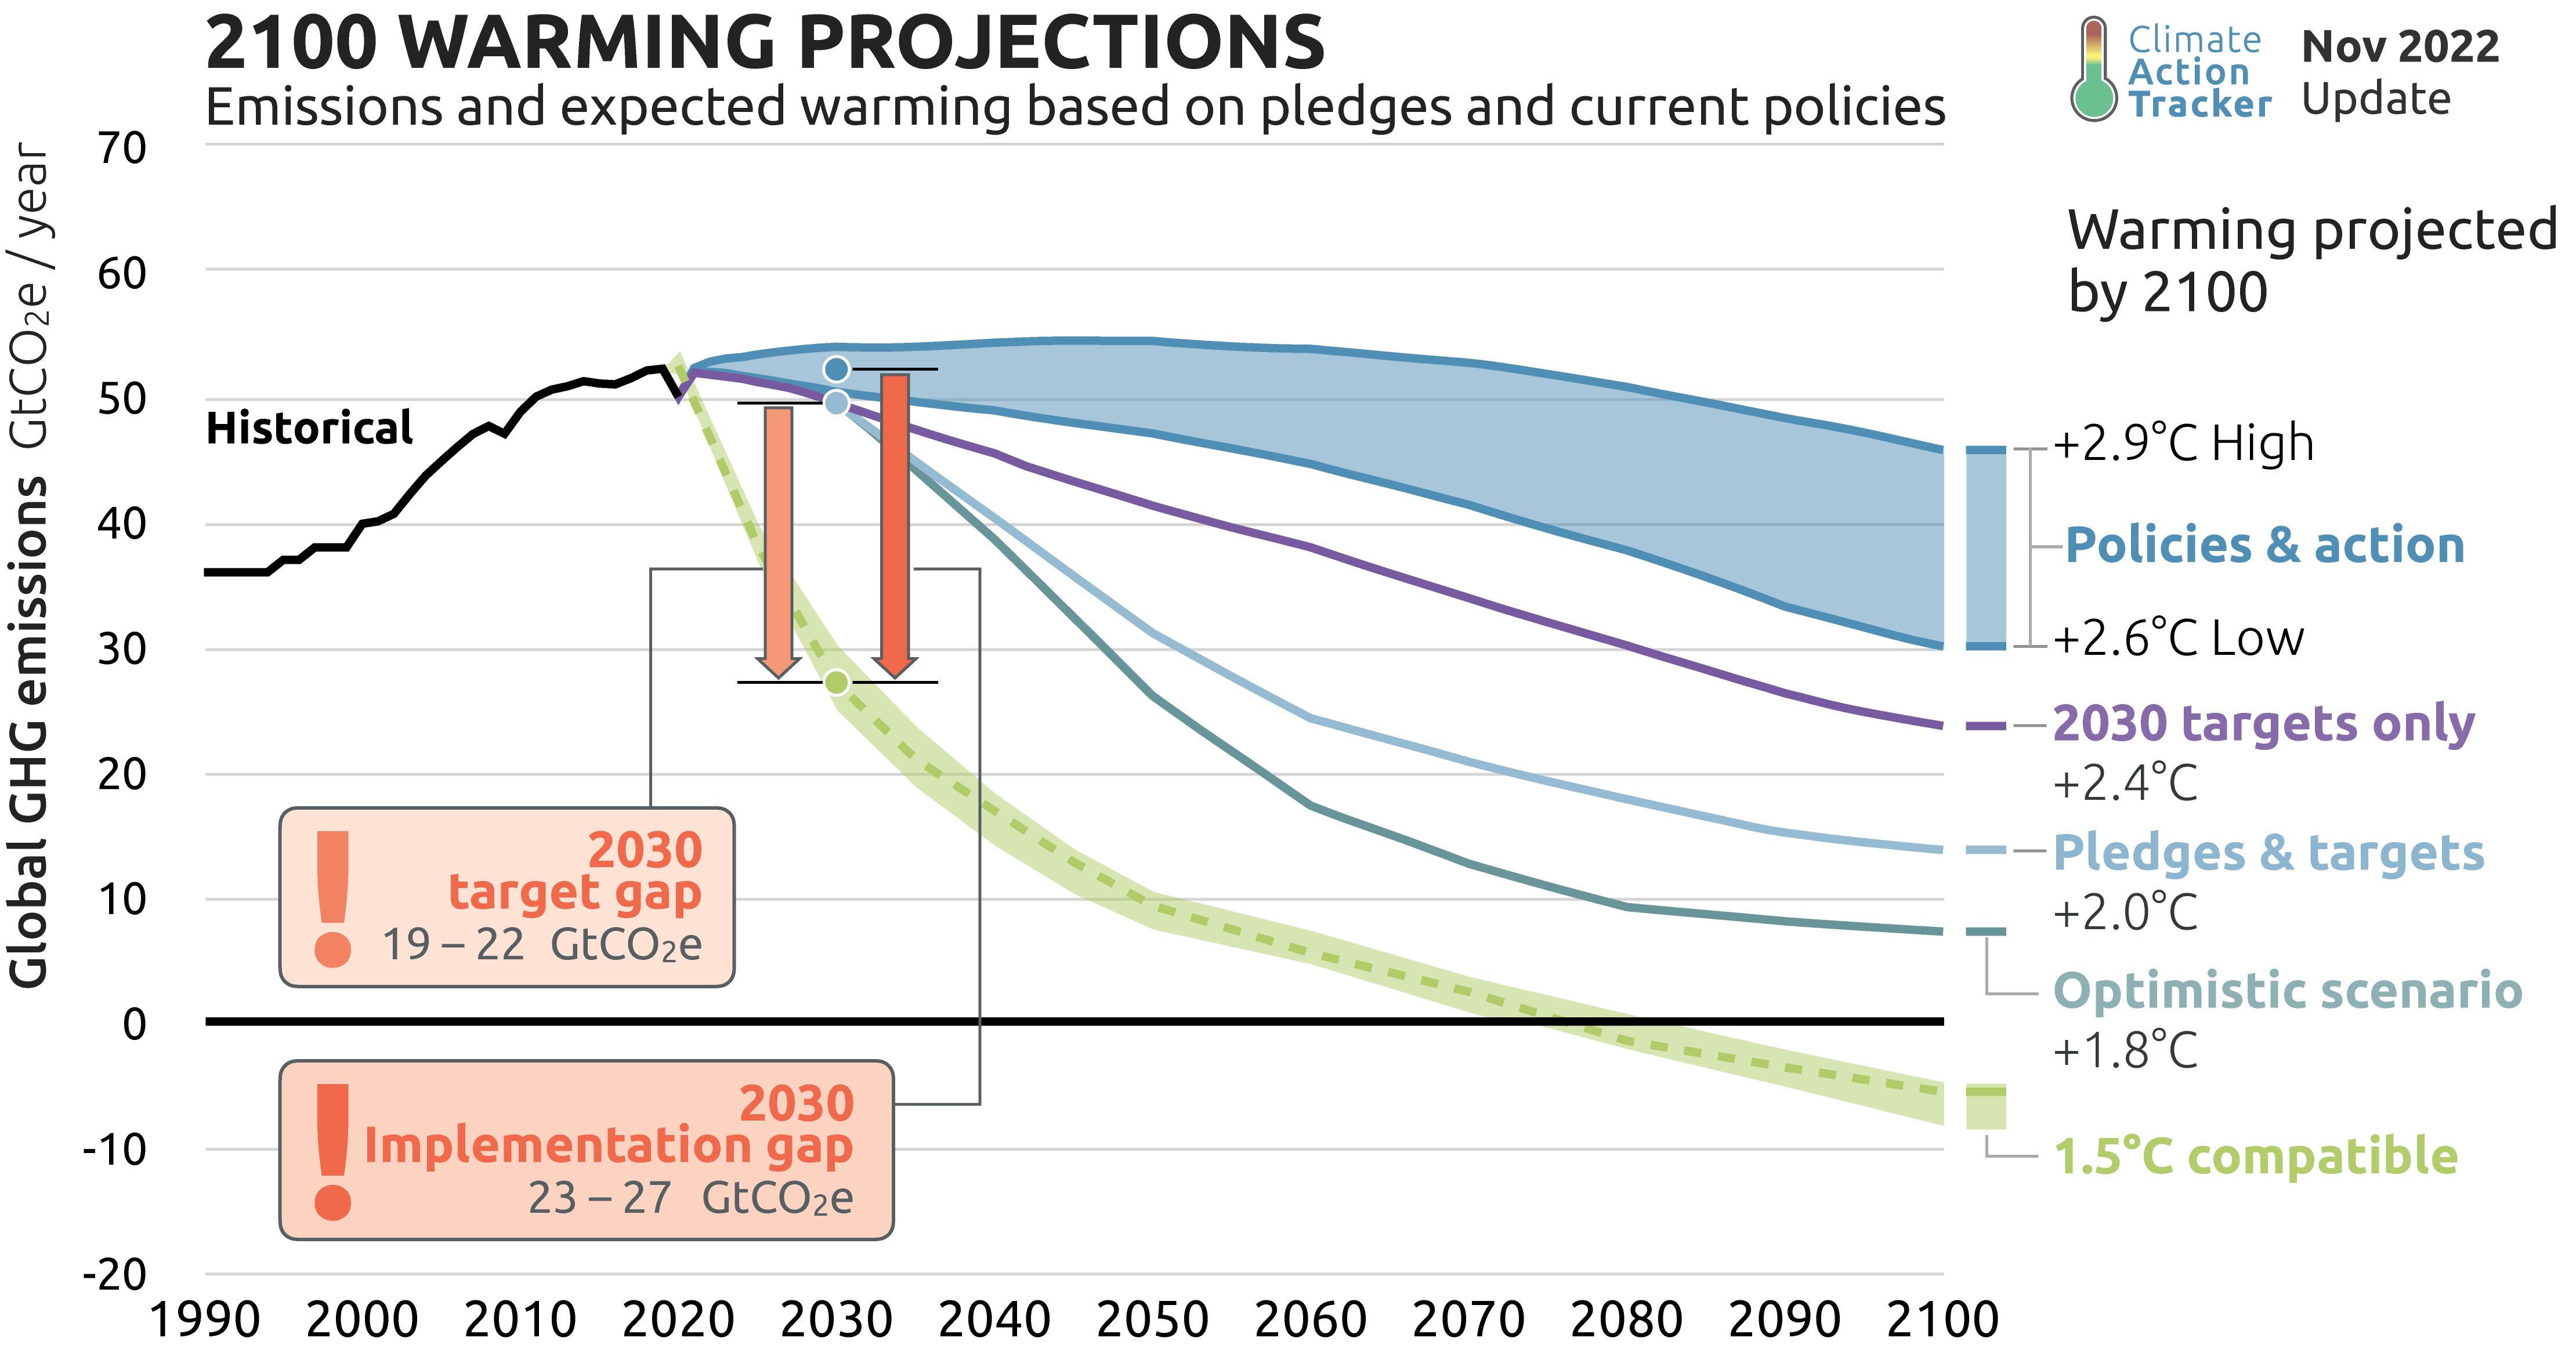
\includegraphics[scale=0.09]{Images/Related_works/Emissions_2022-11.png}
    \caption{Estimated global GHG emissions \cite{tracker2022projections}.}
    \label{fig:ghg_cat}
\end{figure}

We have started to feel the impacts of global warming on humanity, such as heatwaves, droughts, and floods, impacting flora and fauna directly \cite{masson2018global, change2022threat}. In a cascade effect, this increases food and water insecurity worldwide \cite{change2022threat, doi:10.1126/science.1239402}. Also, high temperatures increase mortality, impact labor productivity, impair learning, increase adverse pregnancy outcomes possibility, increase conflict, hate speech, migration, and infectious disease spread \cite{lenton2023quantifying}. Therefore, an increase of the temperature by 2.7\degree C as forecasted would impact one-third (22–39\%) of the world's population by 2100 \cite{lenton2023quantifying}. Climate change has already impacted around 9\% of people (>600 million) \cite{lenton2023quantifying}. Reducing global warming from 2.7 to 1.5\degree C results in a $\sim$5-fold decrease in the population exposed to unprecedented heat (mean annual temperature $\geq$29\degree C) \cite{lenton2023quantifying}. Thus, all sectors must reduce their GHG emissions as much as possible.

Information and Communication Technology is one of these sectors which has accelerated growth in the last 70 years. Unesco defines ICT as \cite{unesco2009guide}:

\begin{quote}
    ``Information and communication technologies (ICT) is defined as a diverse set of technological tools and resources used to transmit, store, create, share or exchange information. These technological tools and resources include computers, the Internet (websites, blogs, and emails), live broadcasting technologies (radio, television, and webcasting), recorded broadcasting technologies (podcasting, audio and, video players, and storage devices), and telephony (fixed or mobile, satellite, visio/video-conferencing, etc.).''
\end{quote}

Regarding the ICT role in GHG emissions, the global share is around 1.8\%-2.8\%, or 2.1\%-3.9\% considering the supply chain pathways in 2020 \cite{freitag2021climate}. The situation tends to get even worst, driven by the boom in Internet-connected devices. A Cisco report indicates that the Internet had 3.9 billion users in 2018 \cite{cisco2020cisco}. The same report predicts an increase to 5.3 billion in 2023 (66 percent of the global population). Also, they predicted 3.6 networked devices per capita in 2023, up from 2.4 networked devices per capita in 2018. However, International Telecommunication Union (ITU), a United Nations specialized agency for ICTs, indicates that we arrived at 5.3 billion connected users in 2022 due to the COVID-19 pandemic \cite{ITU2022}. But will the growth in internet users increase GHG emissions? Andrae and Edler \cite{andrae2015global} and Belkhir and Elmeligi \cite{belkhir2018assessing} agree that this growth could lead to an increase in GHG emissions. Figure \ref{fig:projections_ICT} shows the predictions of both works.

\begin{figure}[!htb]
    \centering
    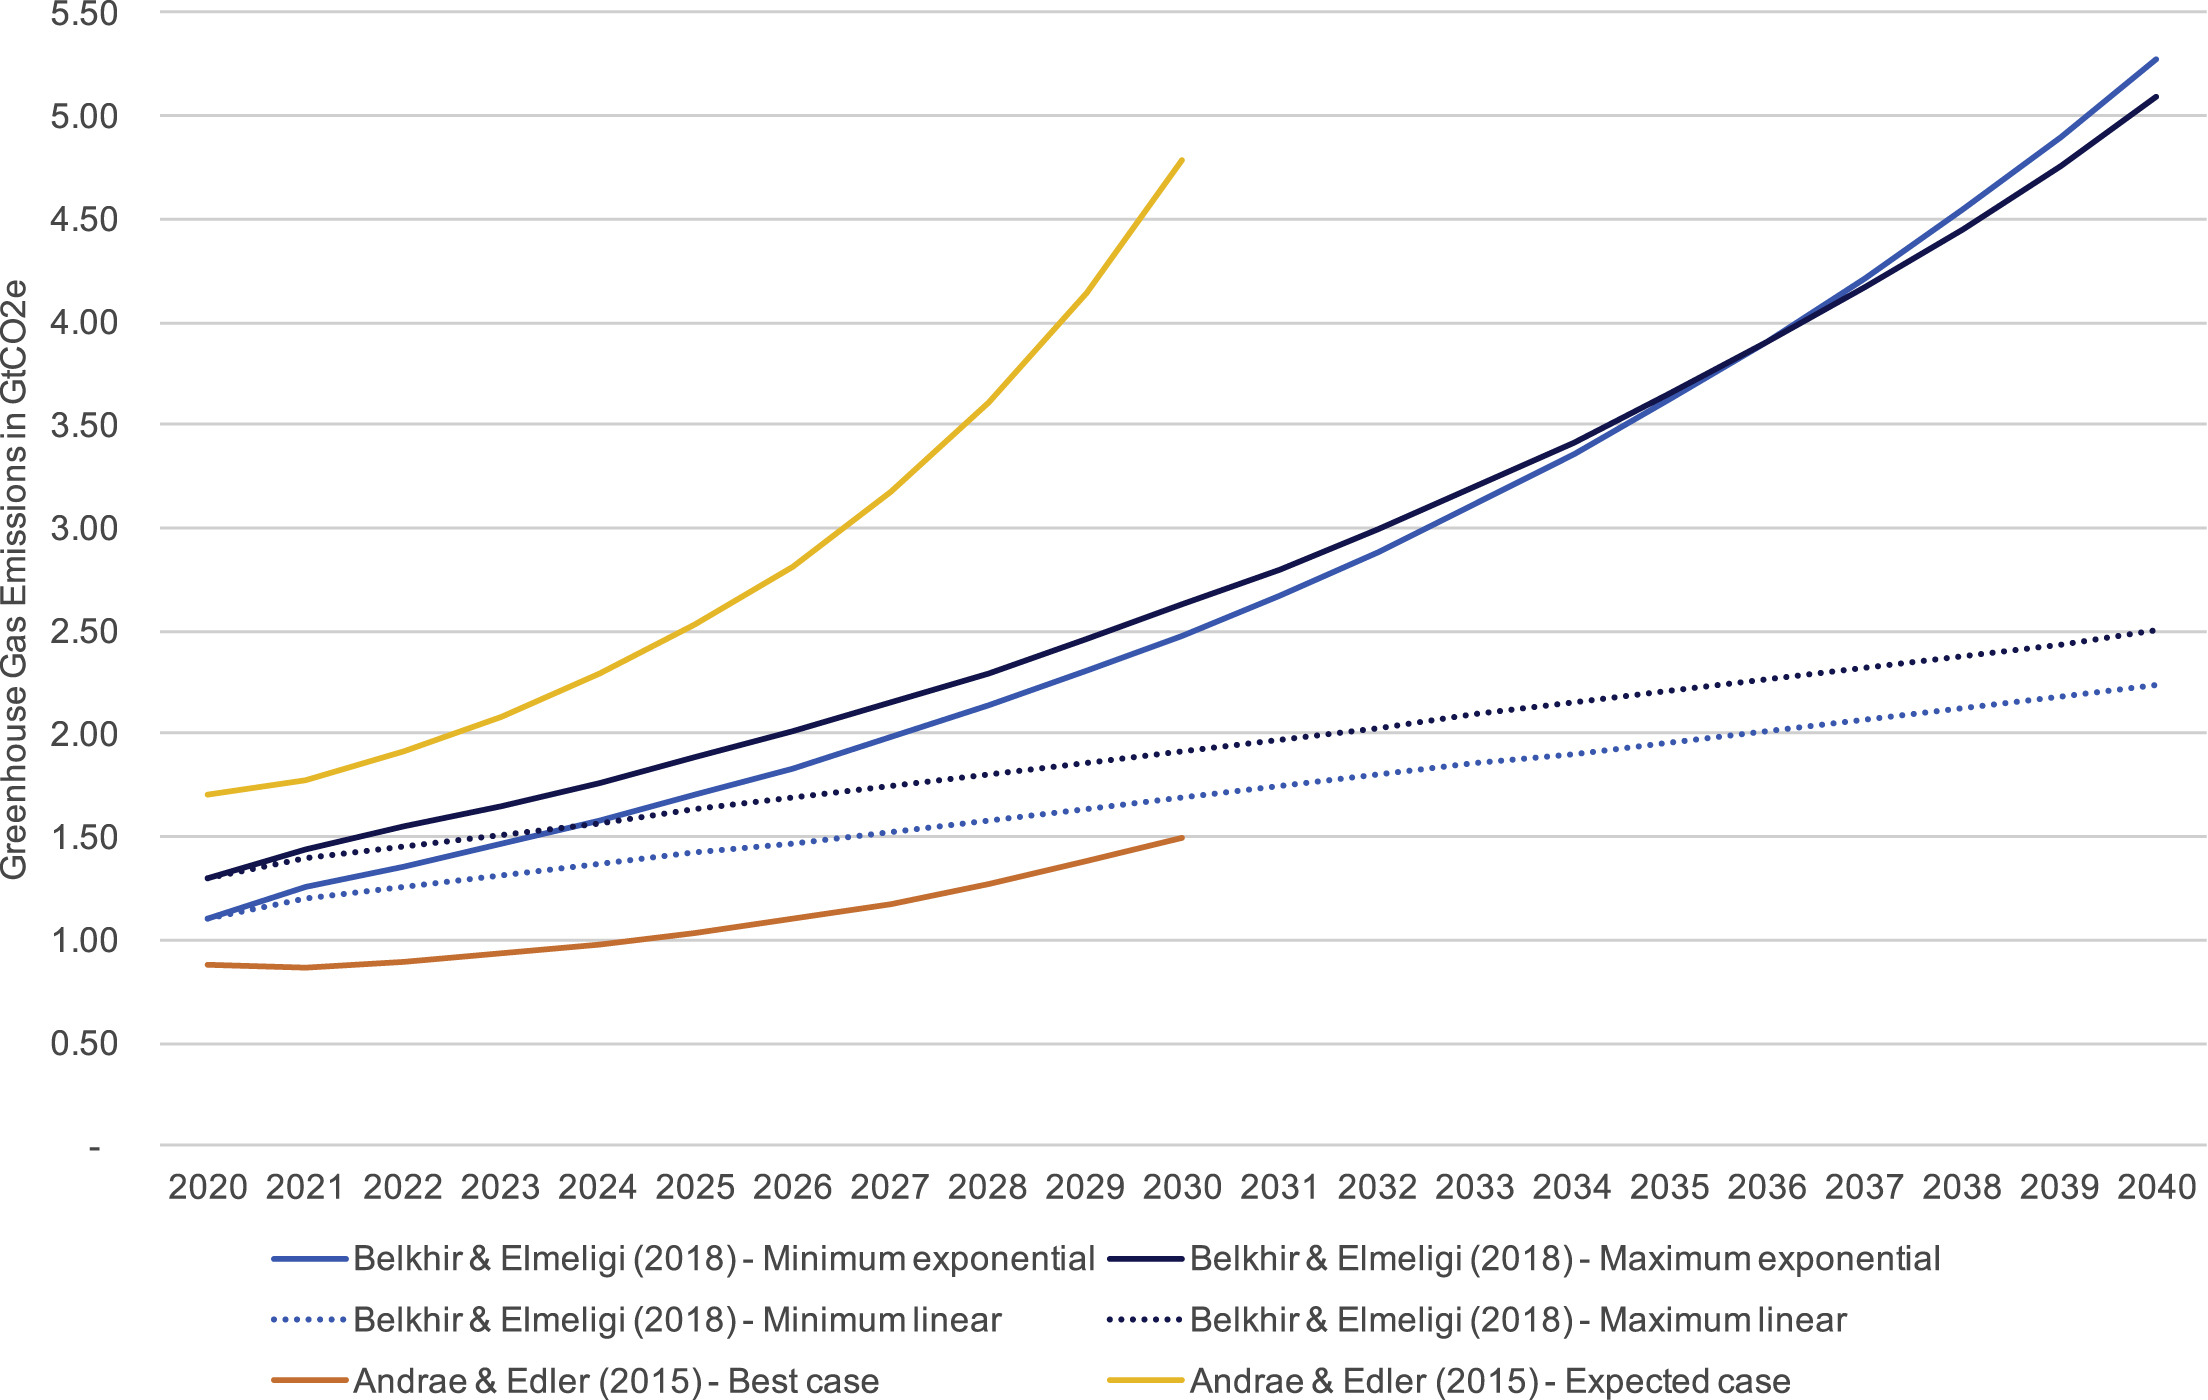
\includegraphics[scale=1]{Images/Related_works/gr4_lrg.jpg}
    \caption{Projections of ICT's GHG emissions from 2020 \cite{freitag2021climate}.}
    \label{fig:projections_ICT}
\end{figure}

This figure illustrates the contraction in the Paris Agreement demand and the predictions about usage in the ICT sector. In all forecasts of Figure \ref{fig:projections_ICT}, the tendency is emissions growth. However, ICT needs to reduce its emissions drastically. Figure \ref{fig:stable_emissions_ICT} illustrates the carbon emission share if the ICT stays at the same level as 2020 and the other sectors decrease their emissions. Without changes, ICT would have 35.1\% of global emissions in 2050. So, ICT must move towards reducing its emissions. Figure \ref{fig:estimations_ICT} presents the estimations of ICT's GHG emissions for 2015 and 2020 from different authors. This figure breaks down these emissions into different components. One of them, with a good share in some cases, is Data centers. IBM defines the data center as ``A data center is a physical room, building or facility that houses IT infrastructure for building, running, and delivering applications and services, and for storing and managing the data associated with those applications and services'' \cite{datacenterIBM}. The International Energy Agency (IEA) defines data center as \cite{centres2022data}:
\begin{quote}
    ``Data centers are facilities used to house networked computer servers that store, process and distribute large amounts of data. They use energy to power both the IT hardware (e.g., servers, drives, and network devices) and the supporting infrastructure (e.g., cooling equipment).''
\end{quote}

\begin{figure}[!htb]
    \centering
    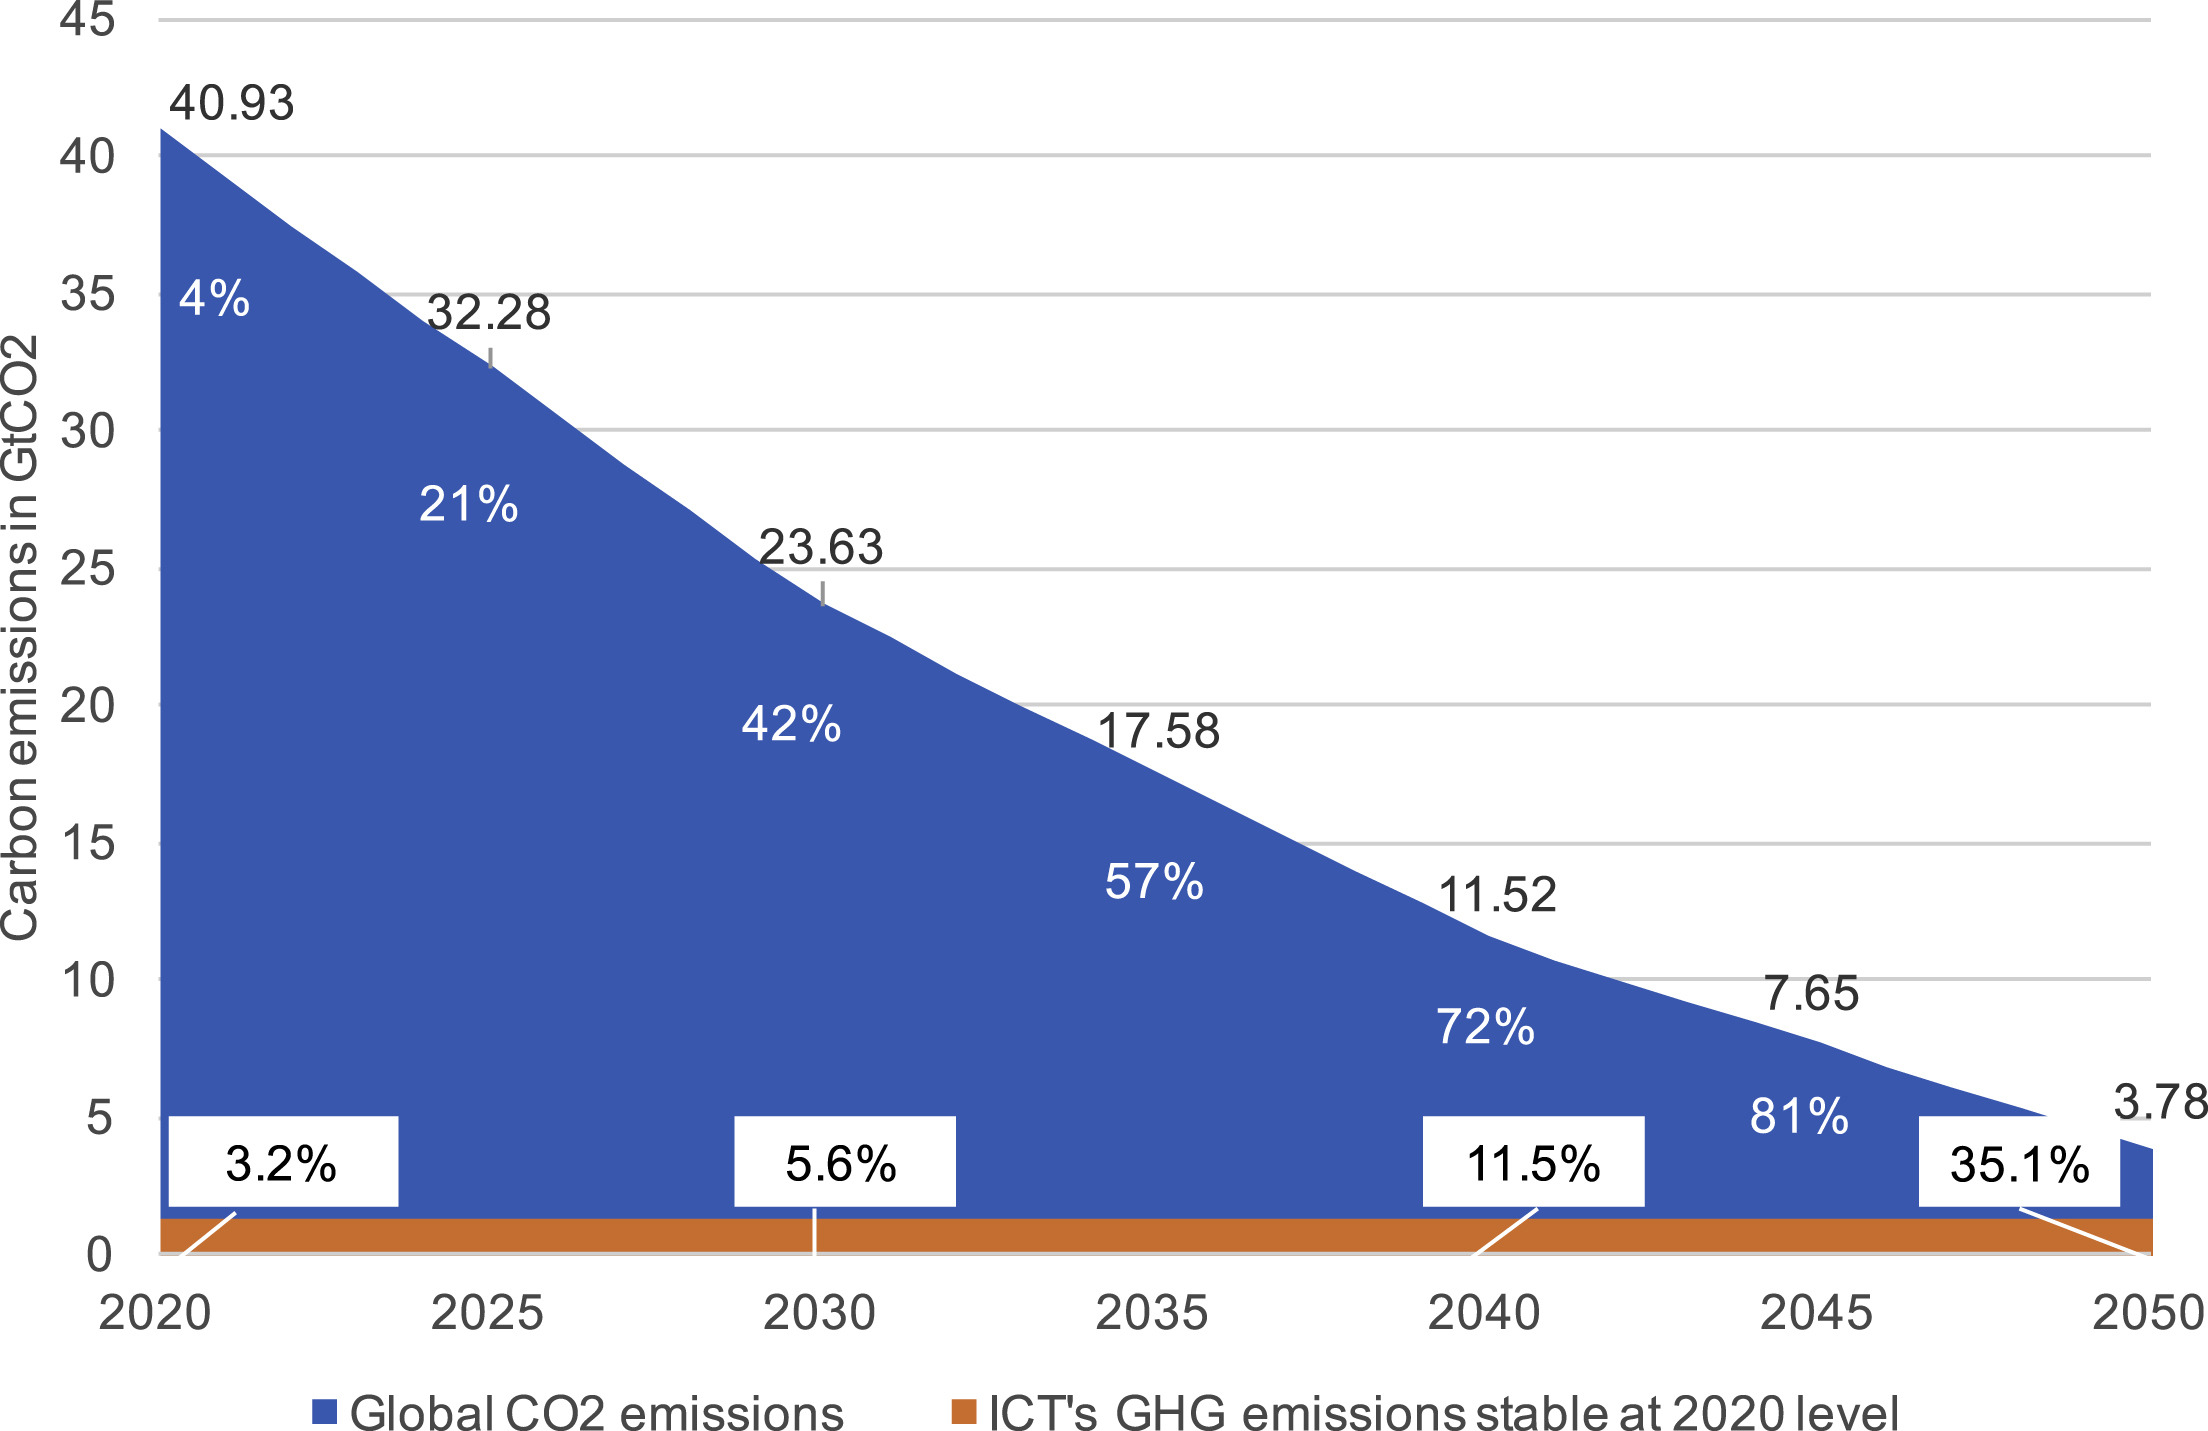
\includegraphics[scale=0.8]{Images/Related_works/gr6_lrg.jpg}
    \caption{ICT's emissions, assuming the 2020 level remains stable until 2050, and global CO2 emissions reduced in line with 1.5\degree C \cite{freitag2021climate}.}
    \label{fig:stable_emissions_ICT}
\end{figure}

\begin{figure}[!htb]
    \centering
    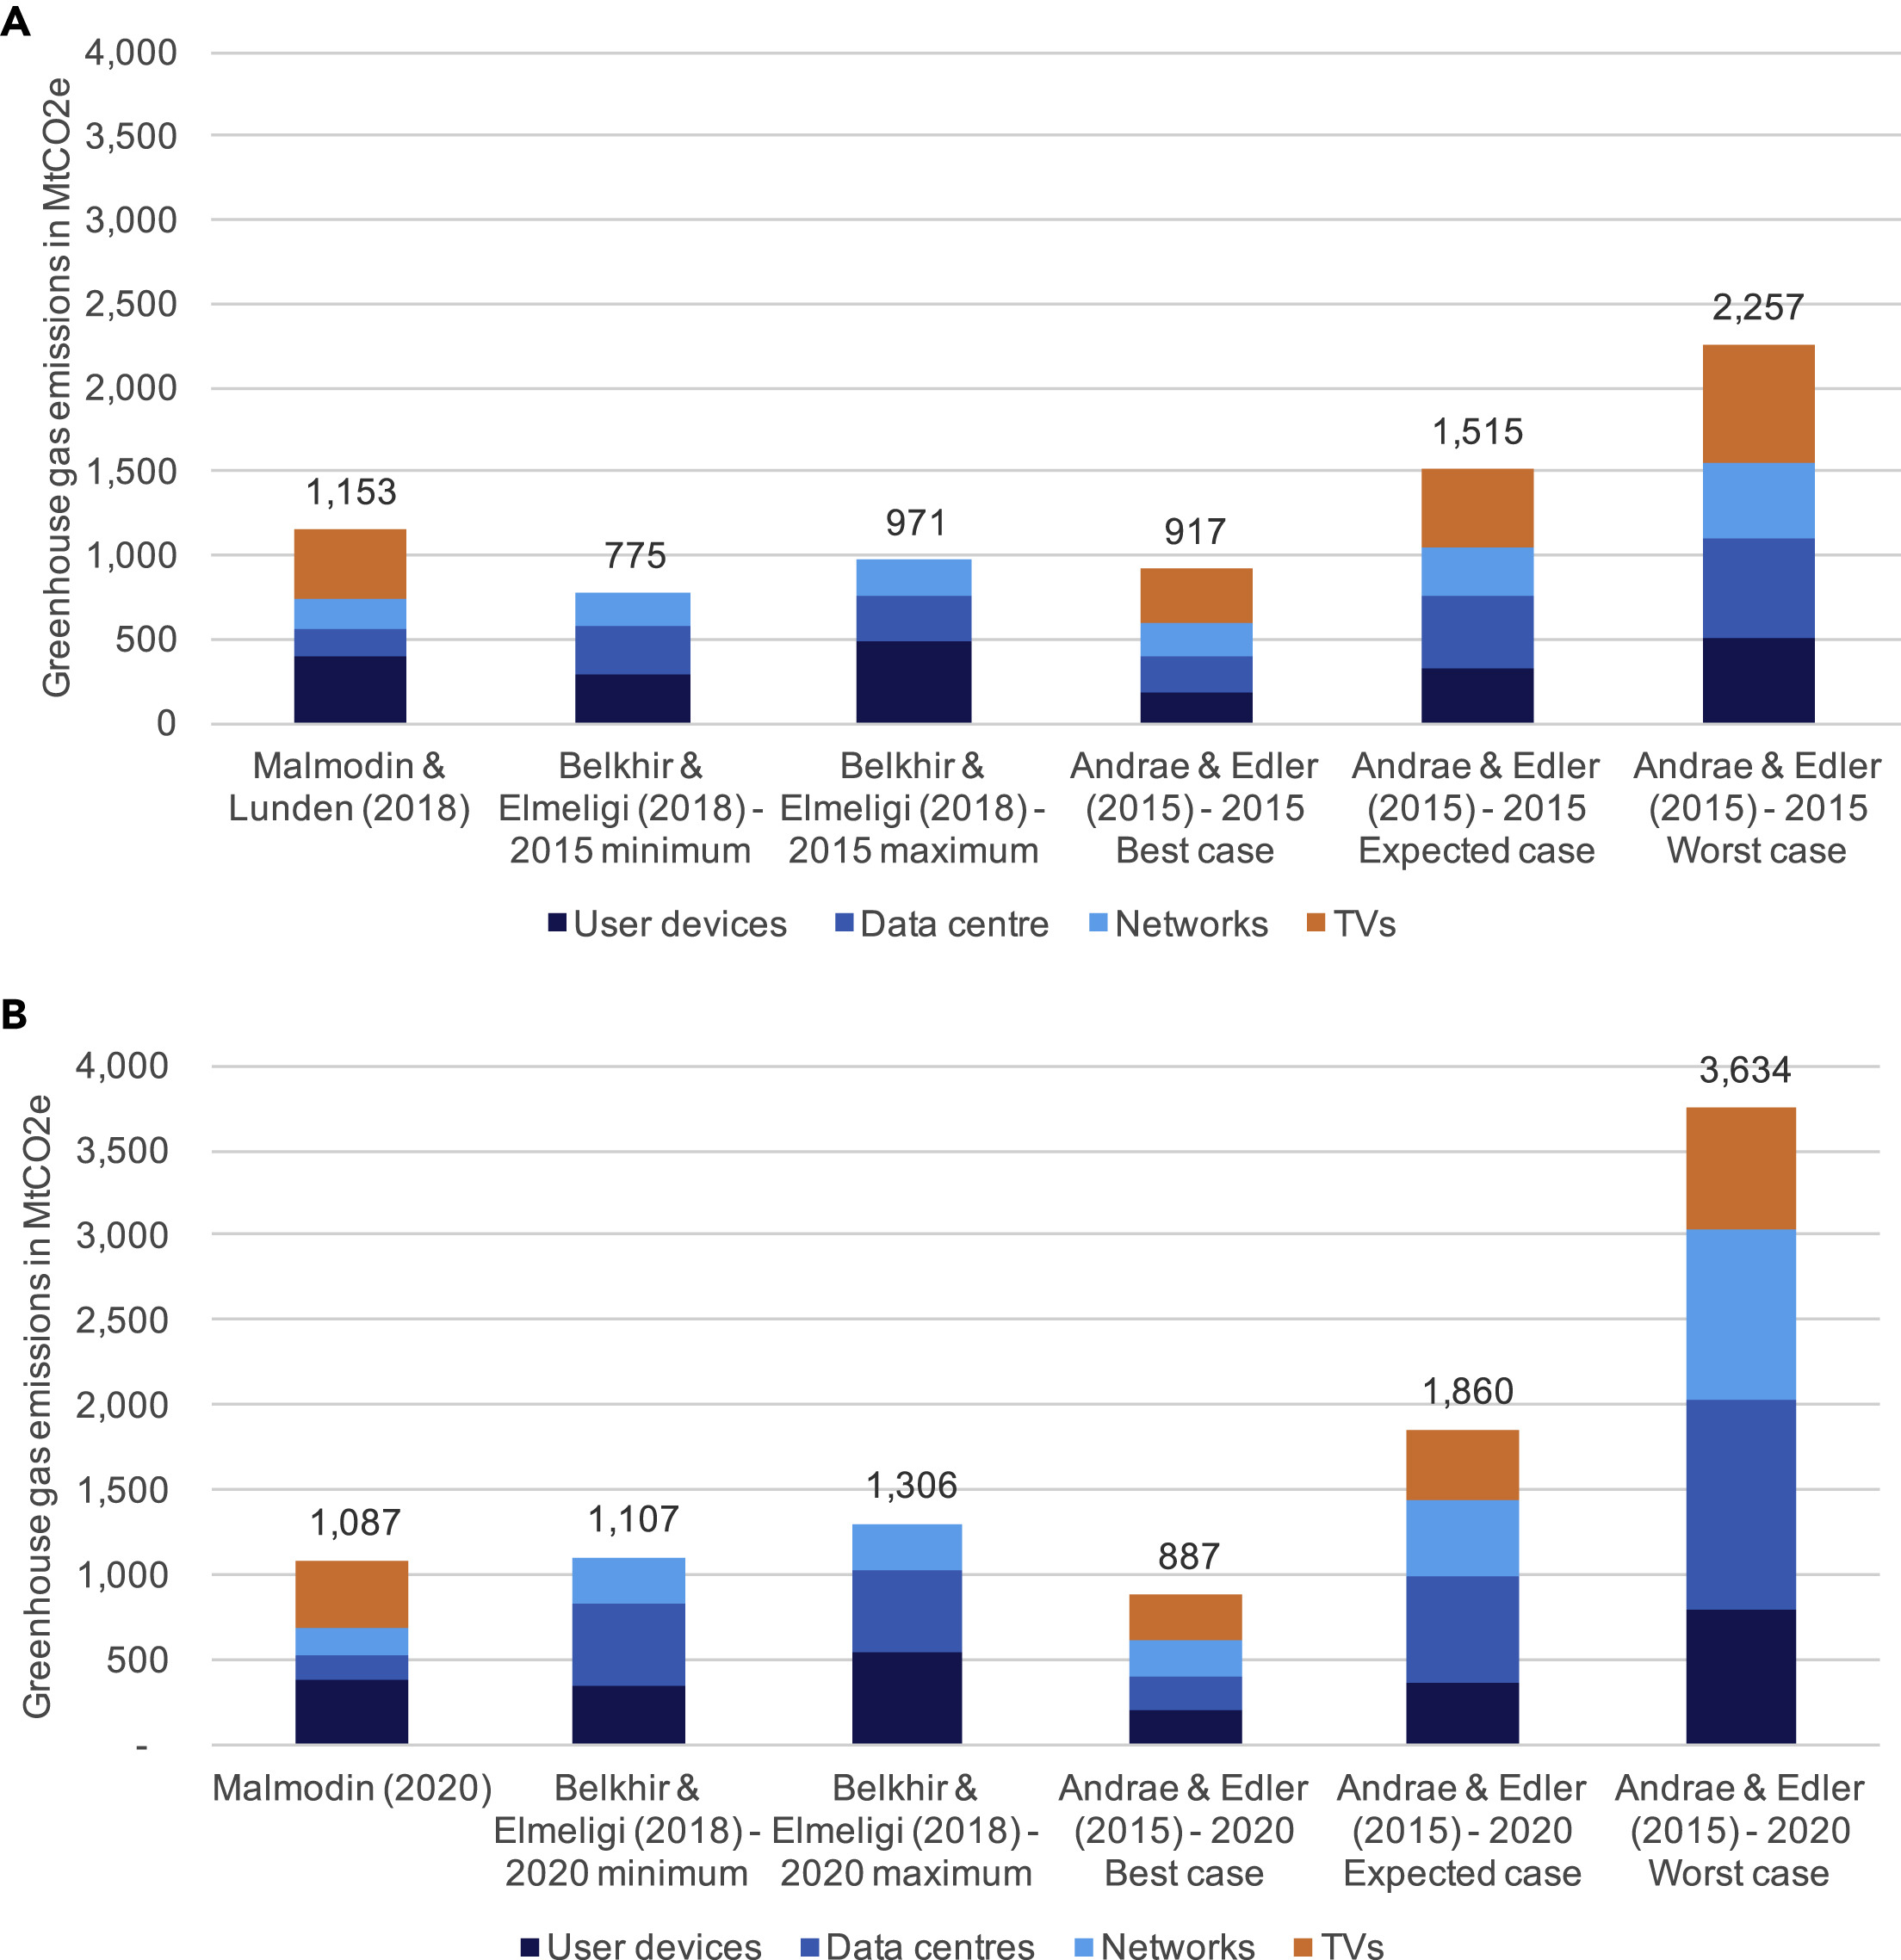
\includegraphics[scale=0.8]{Images/Related_works/gr2_lrg.jpg}
    \caption{Estimations for global ICT’s GHG emissions in 2015 and 2020 \cite{freitag2021climate}. The authors consolidated the works from \cite{belkhir2018assessing, andrae2015global, malmodin2018energy, Malmodin2020}.}
    \label{fig:estimations_ICT}
\end{figure}

Data centers are very energy consumers. IEA published an article indicating that data centers and networks were responsible for almost 1\% of energy-related GHG emissions in 2020 \cite{centres2022data}. Also, Google data centers consumed the same amount of energy as the entire city of San Francisco in 2015 \cite{khan2018exploiting}. Global data center electricity use in 2021 was 220-320 TWh, corresponding to 0.9-1.3\% of the global demand \cite{centres2022data}. For example, the domestic electricity consumption of Italy was 300 TWh in 2021 \cite{ElectricityDomesticConsumption}. In Ireland, electricity consumed by data centers went from 5\% of the total electricity consumption in 2015 to 14\% in 2021 \cite{IrelandDatacenter}. Denmark predicts to triple data center consumption, corresponding to 7\% of the country’s electricity use \cite{DenmarkDatacenter}.

Despite the strong growth in demand, data center energy usage has only moderately grown \cite{centres2022data}. A reason that explains it is the improvements in IT hardware energy consumption \cite{centres2022data}. These improvements allowed a boost in microchips' speed with a reduction in their power consumption, letting big data center companies cope with the peak in demand. Gordon Moore predicted in 1965 (Moore's law) that \cite{moore1965cramming}:

\begin{quote}
    ``The complexity for minimum component costs has increased at a rate of roughly a factor of two per year. Certainly over the short term this rate can be expected to continue, if not to increase. Over the longer term, the rate of increase is a bit more uncertain, although there is no reason to believe it will not remain nearly constant for at least 10 years.''
\end{quote}

Even if he predicted it just until 1975, it is the case nowadays. However, the future is uncertain, and the community is divided to confirm continuous efficiency improvements \cite{freitag2021climate}. While Andrae and Edler \cite{andrae2015global} and Belkhir and Elmeligi \cite{belkhir2018assessing} expected an ending in power-consuming improvements (indicated in Figure \ref{fig:projections_ICT}), Malmodin and Lundén \cite{malmodin2018energy} are more optimistic. They suggest that ICT’s carbon footprint in 2020 could halve by 2030. To achieve that, he considers two key factors. First, the improvements will continue. Second, the migration to renewable sources.

% \begin{itemize}
%     \item Present the numbers of global warming generally;
%     \item Present the predictions about the global warming;
%     \item Introduce the role of ICT generally;
%     \item Write about data center impact;
% \end{itemize}

\section{Renewable Energy Sources}

The ICT migration to renewable energy sources (RES) is one of the factors that helped reduce the growth in GHG emissions despite the rapidly growing demand for digital services \cite{centres2022data}. RES is one of the principal solutions to decarbonize electrical production \cite{olabi2022renewable, rostirolla2022survey}. RES is also named green energy, in contrast to brown energy from fossil fuels. Basically, RES generates energy from natural sources, such as solar, wind, geothermal, hydropower, wave and tidal, and biomass \cite{augustine2012renewable, panwar2011role, rostirolla2022survey, UNREnewable, gross2003progress}. These natural sources have a low impact on GHG emissions. For example, manufacturing is the stage with higher emissions for wind and solar \cite{amponsah2014greenhouse}. So, these components could produce energy with no or low GHG emissions. The renewable term comes from the idea that these sources are constantly replenished. On the other hand, fossil fuels are non-renewable because they need hundreds of millions of years to develop. In the Net Zero Emissions by 2050 Scenario, RES is responsible for one-third of the reductions between 2020 and 2030 \cite{renewables2022}. Some countries focus on nuclear power plants to produce energy \cite{kunsch2014nuclear}. Even if nuclear power is a low carbon emissions energy source, it introduces the risk of accidents and environmental impacts of radioactive wastes \cite{kunsch2014nuclear}.

The biggest challenge of implementing RES is its intermittence \cite{rostirolla2022survey}. Since RES production comes from nature, it depends on the climate conditions. For example, there is no power production from solar during the night. There are two approaches to reducing brown usage: on-site and off-site generation \cite{ren2012carbon}. On-site generation uses local renewable resources, and off-site takes resources available on the grid. In an off-site generation, it is not possible to guarantee that the incoming energy is from RES since the grid mixes all types of power generation \cite{rostirolla2022survey}. Giant cloud providers (e.g., Google, Amazon, and Facebook) invest in solar and wind power plants in an off-site approach \cite{Masanet984, branscombe2020google, amazon2023}. So, they could say that, on average, they provide RES to the grid with the same amount that they expend. However, they transfer the RES uncertainty problem to third parties \cite{rostirolla2022survey}. For example, in a case with a peak in demand, they will use the power from the grid, renewable or not. So, they are still non-renewable-dependent.

\section{Renewable-only Data center}
Since data centers have a controlled infrastructure, they are a good target to migrate to a renewable-only environment \cite{rostirolla2022survey}. However, creating a non-renewable independent data center imposes several challenges. In this kind of data center, all the generation is on-site without backup from the grid. Nevertheless, the production and demand can not match. Figure \ref{fig:load_production} exemplifies the mismatch between the power demanded by a data center and power generation. This mismatch requires a production (electrical) or a load (IT) shift. We will present both electrical and IT elements needed for a renewable-only data center.

\begin{figure}[!htb]
    \centering
    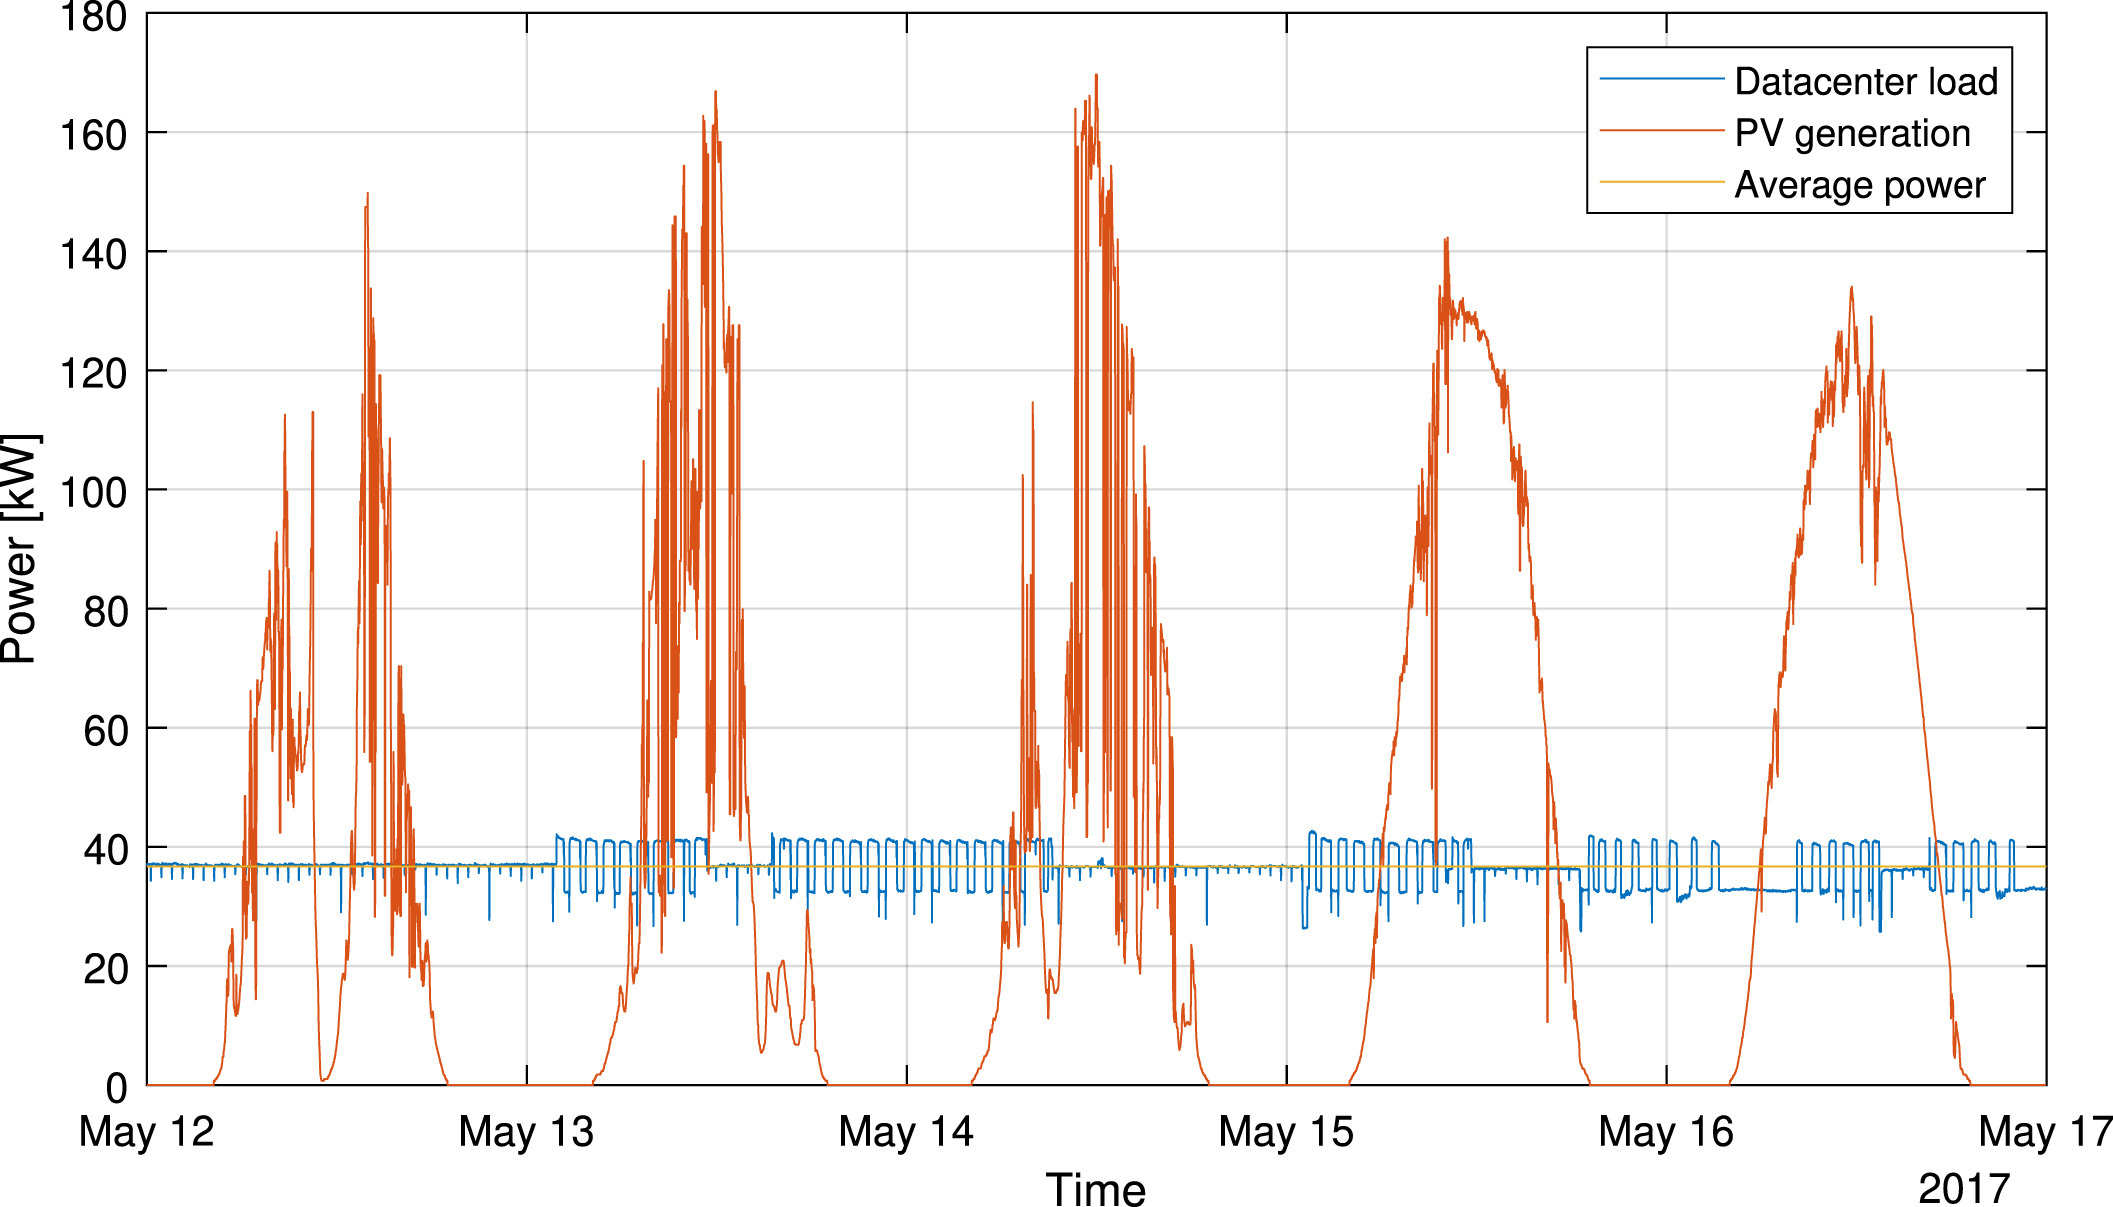
\includegraphics[scale=1]{Images/Related_works/load_production.jpg}
    \caption{Comparison of small data center load and the generation from a theoretical photovoltaic in Belfort, France. Both load and production have the same average value \cite{rostirolla2022survey}.}
    \label{fig:load_production}
\end{figure}

% \begin{itemize}
%     \item Explain the possibility of applying renewable in data centers;
%     \item Present the challenges in a renewable-only data center;
% \end{itemize}

\subsection{Electrical elements}
\label{sec:related_work_electrical_elements}
As mentioned before, different renewable sources can generate power. We focus on wind and solar since they were the most prominent in the past few years \cite{renewables2022}. For wind turbines, the wind speed is crucial. Equation \ref{equ:wind_turbines} gives the power output $P_{WT}(t)$ at the moment $t$ of a wind turbine, given the wind speed $v$ \cite{garcia2006wind, dong2016optimal, maleki2015optimal}.

\begin{equation}
    \label{equ:wind_turbines}
    P_{WT}(t) = \begin{cases}
        0 & v \leq v_{in} \text{ or } v(t) > v_{out} \\
        P_{WT,rated} \times \frac{v(t) - v_{in}}{v_{rated} - v_{in}} & v_{in} < v(t) \leq v_{rated} \\
        P_{WT,rated} & v_{rated} < v(t) \leq v_{out}
    \end{cases}
\end{equation}

Where:
\begin{itemize}
    \item $P_{WT}(t)$: Power generated by a wind turbine (kW);
    \item $v$: Wind speed (m/s);
    \item $v_{in}$: Cut-in wind speed (m/s);
    \item $v_{out}$: Cut-out wind speed (m/s);
    \item $v_{rated}$: Speed related to wind turbine nominal power (m/s);
    \item $P_{WT,rated}$: Wind turbine nominal power (kW).
\end{itemize}

If the wind speed $v$ is lesser or equal to the cut-in $v_{in}$  or greater than the cut-out $v_{out}$, it does not produce power. It tests the cut-out $v_{out}$ to protect the generator. If the speed $v$ is greater than the cut-in $v_{in}$ and lesser or equal to the rated speed $v_{rated}$, it generates proportionally to the rated power $P_{WT,rated}$ and rated speed $v_{rated}$. Finally, if the speed $v$ is greater than the rated speed $v_{rated}$ and lesser or equal to the cut-out $v_{out}$, it produces constant power $P_{WT,rated}$. 

Regarding solar production, the photovoltaic (PV) system uses solar panels to generate power from solar irradiance. Equation \ref{equ:panel_solar_with_temperature} demonstrates how to calculate the output power of a solar panel $P_{pv}(t)$ \cite{maleki2015optimal, sinha2015review, dong2016optimal}.

\begin{equation}
    \label{equ:panel_solar_with_temperature}
    P_{pv}(t) = P_{R,PV} \times (R / R_{ref}) \times \eta_{PV}
\end{equation}

Where:
\begin{itemize}
    \item $P_{pv}(t)$: Power generated by each PV panel (W);
    \item $P_{R,PV}$: PV panel Nominal power (kW);
    \item $R$: Solar irradiance (W/$m^{2}$);
    \item $R_{ref}$: solar irradiance at reference conditions. Usually set as 1000 (W/$m^{2}$) \cite{dong2016optimal};
    \item $\eta_{PV}$: PV efficiency.
\end{itemize}

Regarding PV efficiency $\eta_{PV}$, it can consider the temperature of the solar panel \cite{sinha2015review, maleki2015optimal}. However, some works simplify it by applying a constant value \cite{dong2016optimal, haddad2019mixed}. Equations \ref{equ:wind_turbines} and \ref{equ:panel_solar_with_temperature} demonstrate that both wind turbines and solar panels depend on wind speed and solar irradiance, respectively. So, the weather conditions drive how much power both can generate. 

Due to the weather intermittence, it is necessary to introduce storage elements. These storage elements allow for shifting generation and consumption over time \cite{rostirolla2022survey}. For example, power coming from wind turbines during the night can be stored and used during the day. Big companies are investing in massive storage elements. An example is Google which is planning a 350 MW solar plant in Nevada connected to a storage system of 280 MW \cite{branscombe2020google}. There are different types of storage with advantages and drawbacks \cite{wang2012energy}. One of them is hydropower and underground compressed air storage. However, this kind of storage is very geographical, geological, and terrain dependent, which makes it inappropriate to use in data centers \cite{rostirolla2022survey}. Another type is the very short-term storage such as flywheels or supercapacitors. These storages can output and absorb energy over ms to minutes \cite{wang2012energy}. They are very suitable for maintaining power stability but not for storing energy for a larger time horizon (e.g., hours or days) \cite{rostirolla2022survey}. In this thesis, we focus on the batteries and Hydrogen Storage System (HSS).

Batteries are electrochemical devices that store energy in chemical form \cite{rostirolla2022survey, yilanci2009review, wang2012energy}. They are very reactive because they do not need a warm-up to store/generate power. Batteries are good for short-term storage scenarios (e.g., several hours, day/night cycles) \cite{rostirolla2022survey}. However, they are inappropriate for longer periods due to their self-discharge rate and low energy density \cite{rostirolla2022survey, yilanci2009review}. Historically, Uninterruptible Power Supply (UPS) added batteries to avoid the server's blackout, doing a soft shutdown that avoids several problems, such as data loss, data corruption, work loss, etc. A problem with batteries is the degradation in capacity and performance over time, requiring battery replacement \cite{rostirolla2022survey}. A way to extend battery life is by avoiding charging/discharging too extensively \cite{xu2016modeling}. There are some methods to model the energy level inside the battery, such as energy-based, Current-based, or State of Charge \cite{rostirolla2022survey}. We focus on the State of Charge since it represents the percentage of energy inside the battery according to its capacity (e.g., 100\% means battery full and 0\% dry). \citeauthor{xu2016modeling} present results showing that maintaining SoC at a narrow range reduces battery degradation \cite{xu2016modeling}. However, using a narrow range would reduce the battery's effectiveness because it can deliver less energy to deal with intermittence. So, the battery SoC must be maintained within a range considering this trade-off. Equations \ref{equ:battery_energy} and \ref{equ:battery_state_of_charge} demonstrate how to calculate the State of Charge \cite{haddad2019mixed}. 

\begin{equation}
    \label{equ:battery_energy}
    E_{bat}(t) = (E_{bat}(t-1) \times (1 - \sigma)) + (P_{ch}(t-1) \times \eta_{ch} \times \Delta t) - (\frac{P_{dch}(t-1)}{\eta_{dch}} \times \Delta t)
\end{equation}
\begin{equation}
    \label{equ:battery_state_of_charge}
    SoC(t) = \frac{E_{bat}(t)}{B_{size}} \times 100
\end{equation}

Where:
\begin{itemize}
    \item $\Delta t$: Duration of $t$ (h);
    \item $E_{bat}(t)$: Energy in the battery at instant $t$ (kWh);
    \item $P_{ch}(t-1)$: Charging power (kW);
    \item $P_{dch}(t-1)$: Discharging power (kW);
    \item $\sigma$: Battery self-discharge rate (\%);
    \item $\eta_{ch}$: Battery charge efficiency (\%);
    \item $\eta_{dch}$: Battery discharge efficiency (\%);
    \item $B_{size}$: Battery size (kWh);
    \item $SoC(t)$: State of Charge at instant $t$ (\%);
\end{itemize}

We can divide Equation \ref{equ:battery_energy} into three parts. The first part ($E_{bat}(t-1) \times (1 - \sigma)$) calculates the natural self-discharge, ignoring charging or discharging the battery. The second part ($P_{ch}(t-1) \times \eta_{ch} \times \Delta t$) computes the energy stored in the battery according to the charging power. The last part ($\frac{P_{dch}(t-1)}{\eta_{dch}} \times \Delta t$) is similar but for discharging. Both charging and discharging are not perfect with some losses given by $\eta_{ch}$ and $\eta_{dch}$. For example, if we charge 1 kW this does not mean that, after one hour, we charge 1 kWh. We will charge $1 kW \times \eta_{ch}$ (where $\eta_{ch} < 1$). Also, we can not charge and discharge the battery simultaneously, so if $P_{ch} > 0$ then $P_{dch} = 0$, and vice-versa \cite{haddad2019mixed}. Equation \ref{equ:battery_state_of_charge} normalizes the SoC to percentage.

Hydrogen, differently from batteries, is more suitable for long-term storage (e.g., over seasons), mainly because it can store large amounts of energy with very low self-discharge \cite{pregger2009prospects}. A big limitation of this kind of storage is the lack of reactivity since it demands a longer warming-up time. Also, it includes performance degradation concerns, low efficiency compared to batteries, high costs, and complicated safety measures \cite{rostirolla2022survey}. Even with all these drawbacks, it is a good solution for storing energy during abundant periods (e.g., summer) and using it during lacking periods (e.g., winter). Three elements compose an HSS: electrolyzer, hydrogen tank, and fuel cell. The electrolyzer produces hydrogen from electricity, according to Equation \ref{equ:hydrogen_electrolyzer} \cite{haddad2019mixed}.

\begin{equation}
    \label{equ:hydrogen_electrolyzer}
    P_{ez}(t) \times \Delta t = \frac{HH_{h_{2}} \times Q_{ez}(t)}{\eta_{ez}}
\end{equation}

Where:
\begin{itemize}
    \item $P_{ez}(t)$: Power put into electrolyzer (kW);
    \item $HH_{h_{2}}$: H2 higher heating value ($kWh / kg$);
    \item $Q_{ez}(t)$: Electrolyzer H2 mass flow (kg);
    \item $\eta_{ez}$: Electrolyzer efficiency (\%);
\end{itemize}

This equation indicates how much hydrogen is added to the tank ($Q_{ez}(t)$) according to the electrolyzer operating power ($P_{ez}(t)$). On the other hand, the fuel cell transforms hydrogen into electricity, according to Equation \ref{equ:hydrogen_full_cell} \cite{haddad2019mixed}.

\begin{equation}
    \label{equ:hydrogen_full_cell}
    P_{fc}(t) \times \Delta t = LH_{h_{2}} \times Q_{fc}(t) \times \eta_{fc}
\end{equation}

Where:
\begin{itemize}
    \item $P_{fc}(t)$: Power delivered by fuel cell (kW);
    \item $LH_{h_{2}}$: H2 lower heating value ($kWh / kg$);
    \item $Q_{fc}(t)$: Fuel cell H2 mass flow (kg);
    \item $\eta_{fc}$: Fuel Cell efficiency (\%);
\end{itemize}

Similarly, this equation indicates how much hydrogen is removed from the tank ($Q_{fc}(t)$) according to the output power of the fuel cell ($P_{fc}(t)$). To calculate the Level of Hydrogen ($LoH(t)$ (kg)) Equation \ref{equ:hydrogen_level} consolidates the result of the electrolyzer and the fuel cell.

\begin{equation}
    \label{equ:hydrogen_level}
    LoH(t) = LoH(t-1) + Q_{ez}(t-1) - Q_{fc}(t-1)
\end{equation}

\subsection{IT elements}
\label{sec:related_work_it_elements}
While electrical elements are power producers (wind turbines and solar panels) or producers/consumers (storage), the IT elements are entirely power consumers. IT power consumption can be divided into two parts: IT hardware (e.g., servers, data storage, and network devices) and supporting infrastructure (e.g., cooling equipment) \cite{centres2022data, dayarathna2015data}. This thesis focus on computing nodes (servers) and scheduling policies on the IT side, so we do not consider data storage, network devices, and supporting infrastructure. There are several articles dealing specifically with these components \cite{dayarathna2015data, orgerie2014survey, zhang2021survey, hammadi2014survey}. The servers are powerful, high-performance machines designed to handle intensive computational tasks and ensure the efficient functioning of various applications and services. They are optimized for reliability, scalability, and performance. Even with these optimizations, they do not have a negligible power consumption \cite{ismail2020computing, orgerie2014survey}.

The server power consumption is divided into two parts: static and dynamic \cite{orgerie2014survey, heinrich2017predicting}. Static power consumption is constant and given by current leakage present in any powered system. Dynamic power is not constant and depends on computing usage. There are different models to estimate power consumption, such as mathematical linear and non-linear, linear regression, lasso regression, support vector machines, etc. Equation \ref{equ:cpu_usage} expresses a mathematical linear representation of static and dynamic power \cite{heinrich2017predicting, ismail2020computing}.

\begin{equation}
    \label{equ:cpu_usage}
    Pcpu(t) = P^{static} + (P^{dynamic} \times u_{cpu})
\end{equation}

Where:
\begin{itemize}
    \item $Pcpu(t)$: Power consumption at moment $t$ (W);
    \item $P^{static}$: Static power consumption (W);
    \item $P^{dynamic}$: Dynamic power consumption (W);
    \item $u_{cpu}$: CPU usage (\%);
\end{itemize}


While \citeauthor{ismail2020computing} indicate that $P^{static}$ can be considered as the power idle \cite{ismail2020computing}, \citeauthor{heinrich2017predicting} demonstrate a slight difference between the power usage at fully idle and when the real $P^{static}$ \cite{heinrich2017predicting}. The work of \citeauthor{heinrich2017predicting} is the base for a well-known data center simulator named Simgrid\footnote{https://simgrid.org/} and its evolutions. This article also indicates that $P^{dynamic}$ depends on the application and the server frequency. Figure \ref{fig:cpu_frequency_consumption} shows the linearization of the power consumption according to the frequency for the same application. Setting different frequencies is possible through the Dynamic Voltage and Frequency Scaling technique. Putting the server at a lower frequency reduces the server's power consumption (as illustrated in Figure \ref{fig:cpu_frequency_consumption}). However, it also decreases the server's speed. Nevertheless, DVFS is a possible solution to reducing energy consumption in moments with lower power available. 

\begin{figure}[!htb]
    \centering
    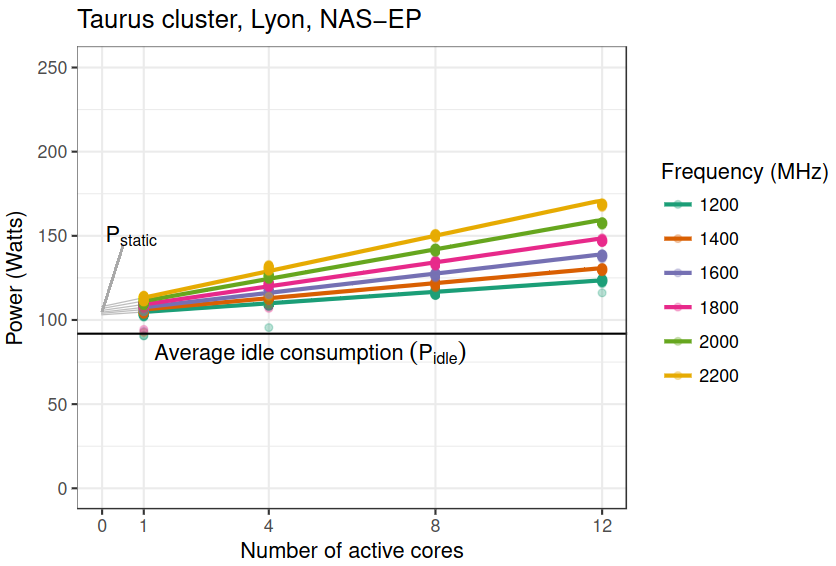
\includegraphics[scale=0.4]{Images/Related_works/cpu_usage.png}
    \caption{Power consumption on a GRID5000 server when running the same application, but varying the frequency and the number of active cores \cite{heinrich2017predicting}.}
    \label{fig:cpu_frequency_consumption}
\end{figure}

Another possibility, more drastic, is putting the server to sleep. In the sleep state, the server is unavailable but consuming its lower power possible. Besides being inaccessible, another consideration in the sleep state is that sleep transitions (on$\rightarrow$off and off$\rightarrow$on) are not instantaneous and waste energy. \citeauthor{rais2018quantifying} present a Dynamic Power Management (DPM) solution \cite{rais2018quantifying}. This DPM estimates a $T_{wait}$ threshold that when the server is idle for more than $T_{wait}$ seconds, it is more energy-efficient to switch the server off. Equation \ref{equ:dpm_waiting_time} represents their idea.

\begin{equation}
    \label{equ:dpm_waiting_time}
    T_{wait} = \max(\frac{E_{OnOff} + E_{OffOn} - (P_{Off} \times (T_{OnOff} + T_{OffOn}))}{P_{idle} - P_{Off}}, (T_{OnOff} + T_{OffOn}))
\end{equation}

Where:
\begin{itemize}
    \item $T_{wait}$: Waiting time before putting the server to sleep (s);
    \item $P_{idle}$: Power consumption when the server is unused, but powered on (W);
    \item $P_{Off}$: Power consumption when the server is off (not null and lower than $P_{idle}$) (W);
    \item $E_{OnOff}$: Energy consumed during the On$\rightarrow$Off transition (J);
    \item $E_{OffOn}$: Energy consumed during the Off$\rightarrow$On transition (J);
    \item $T_{OnOff}$: Time spent by the server on On$\rightarrow$Off (s);
    \item $T_{OffOn}$: Time spent by the server on Off$\rightarrow$On (s);
\end{itemize}


A data center's main objective is to execute users' applications. Running applications in the servers variates the server's CPU usage $u_{cpu}$. Data centers receive plenty of different application types. We can separate these applications into two big categories: services and batch \cite{rostirolla2022survey,da2018modeling}. Services are applications that interact with different clients. These clients make requests answered by a running service. Each request has a low processing time, but the ensemble of these requests can be very CPU-consuming \cite{masdari2020survey}. Also, the service must answer the request as soon as it arrives. On the other hand, batch applications (or parallel jobs \cite{feitelson2014experience}) do not run interactively. While services can run indefinitely, batches have a start and end time. Usually, these applications aim to solve complex problems, such as weather prediction, optimization problems, and simulations, being very long and CPU-consuming \cite{masdari2020survey}. Batch jobs are more flexible considering the moment to execute them, allowing the batch scheduler to define the best moment in the future to run them. Both services and batches demand different approaches and algorithms to deal with them. This thesis focuses on batch high-performance computing (HPC) applications. An HPC job is composed by \cite{rostirolla2022survey, srinivasan2002characterization, takizawa2020effect}:

\begin{itemize}
    \item Submission time: The moment when the user sends the job;
    \item Requested resources: The resources demanded by the job, such as the number of cores, servers, memory, etc;
    \item Estimated execution time or walltime: The user indicates how long the job executes. If the real execution time is equal to the walltime, the scheduler kills the job. 
\end{itemize}

% \begin{itemize}
%     \item Write about the servers;
%     \item Write about the power consumption (e.g., DVFS, on-off, idle, etc);
%     \item Write about the jobs (e.g., types, resources demanded, etc);
% \end{itemize}

\section{Sources of Uncertainty}

After describing renewable-only data center elements, in this section, we detail the sources of uncertainty. First, we start presenting the uncertainty from electrical components due to weather conditions. After that, we describe the uncertainties from server power consumption and HPC jobs. Finally, we discuss the challenges in dealing with all these uncertainties.

\subsection{Weather Uncertainties}
As presented in Section \ref{sec:related_work_electrical_elements}, the objective of the electrical components (solar panels and wind turbines) is to generate power. So, they transform natural renewable resources into energy. Due to the intermittence of these renewable resources, the output power is also intermittent \cite{perez2011managing}. Regarding solar panels, the output power is calculated easily, using Equation \ref{equ:panel_solar_with_temperature}, in a "clear-sky" condition \cite{tuohy2015solar}. "Clear-sky" considers an exposition total of the panels to the sun. However, solar irradiance is impacted by several weather conditions, such as clouds, aerosols, and other atmospheric constituents \cite{tuohy2015solar}. Also, the panel efficiency is temperature dependent. Concerning wind turbines, the power output depends on the wind speed (see Equation \ref{equ:wind_turbines}). The production has lower and higher wind speed thresholds, meaning that even too slow/fast wind will not produce power. 

Due to the renewable intermittence, it is crucial to forecast weather conditions to estimate future power production. Several works propose ways to predict these conditions \cite{tuohy2015solar, soman2010review, sharma2018review, ssekulima2016wind}. Two key terms are important in renewable production: Predictability and Variability \cite{ssekulima2016wind, perez2011managing}. Predictability means the ability to anticipate the availability of a generation resource \cite{perez2011managing}. For example, solar irradiance is more predictable than wind speed because the forecast accuracy on clear days is high, and satellite data tracks precisely the direction and speed of clouds \cite{perez2011managing}. On the other hand, due to the erratic nature of the atmosphere, there is randomness in wind power production \cite{sharma2018review}. Variability indicates the variation over time in production \cite{perez2011managing}. Both wind and solar can vary. For example, the wind has high variability because it will deviate from 0\%–100\% over a day \cite{perez2011managing}. Another element that influences forecast accuracy is the time horizon. For example, the next five minutes are more predictable than the next three days.

% \begin{itemize}
%     \item Describe wind uncertainty;
%     \item Describe solar irradiance uncertainty;
% \end{itemize}

\subsection{Workload Uncertainties}
Workload uncertainties come from two sources: the server's energy consumption and jobs. Estimating the real power consumption of a server is not trivial. Several works try to find a model to describe energy consumption or even apply machine learning to define it \cite{dayarathna2015data}. Even two machines with the same configuration can consume differently \cite{orgerie2010demystifying}. It is also true that each application can have a completely different energy consumption, mainly because they use the CPU differently \cite{orgerie2010demystifying}. Equation \ref{equ:cpu_usage} presents a simplification of server power consumption. However, this equation is still applicable since different servers can have different dynamic ($P^{dynamic}$) and static ($P^{static}$) power. Also, considering that energy consumption is Equation \ref{equ:cpu_usage} integral, different applications can have distinct CPU usage ($u_{cpu}$). Even if the equation is still appropriate, defining its parameters is challenging. For example, the CPU usage ($u_{cpu}$) of a job can vary between executions (e.g., due to different application parameters). Also, new applications do not have records to estimate their usage. Considering the static power ($P^{static}$), it is known that it can vary according to the processor's heat \cite{patterson2008effect}.

Besides impacting server consumption, jobs have their own uncertainties. A workload (ensemble of jobs) can be predicted as a load mass or resource usage (e.g., CPU usage over time) \cite{masdari2020survey, vashistha2020literature}. These predictions indicate the estimated demand load, but the exact jobs' arrival is very difficult to predict. The submission is one of the job uncertainties. In a renewable-only data center, this uncertainty mainly impacts the number of servers available. For example, if a server is available expecting a job, but the job does not come or arrives late, this server wastes energy unnecessarily (e.g., by being idle, turning on/off). The second job uncertainty is the execution time. The scheduler receives jobs with requested resources and walltime. So, the scheduler will find a placement for each job to match the requested resources during the walltime. The walltime is a user expectation of the execution time that can be overestimated \cite{takizawa2020effect}. An overestimated walltime reduces the effectiveness of the scheduler because it will reserver more time than necessary for the job \cite{srinivasan2002characterization, takizawa2020effect}.

% \begin{itemize}
%     \item Power consumption;
%     \item Describe job arrival uncertainty;
%     \item Describe job size uncertainty;
% \end{itemize}

\subsection{Dealing with Uncertainties}
After describing the uncertainties in electrical and IT elements, we present some ways to deal with them. The renewable-only data center global problem is a scheduling problem under power constraints. Therefore, the problem includes:
\begin{itemize}
    \item finding the best moment to start jobs;
    \item increasing power production from energy storage to improve QoS (e.g., running more jobs, avoiding killing jobs, finishing jobs earlier, etc.);
    \item adapting power consumption to dealing with over/underproduction;
    \item starting/stopping servers matching the defined power consumption;
    \item letting battery between the safe state of charge thresholds.  
\end{itemize}

An optimization problem must consider all these elements. We can divide the problem into offline and online. Offline optimization uses predictions (from weather and workload) to optimize the decisions. Some methods are available to estimate power production and demand, such as Artificial Neural Networks, Support Vector Machines, Markov Chains, Regression Models, Autoregressive Models, and a combination of the methods, such as using genetic algorithms to optimize a neural network \cite{vashistha2020literature, masdari2020survey, ssekulima2016wind, sharma2018review, tuohy2015solar}. Then, this optimization finds the best approach to match production and demand (e.g., shifting the load, using more power from batteries, rejecting jobs, etc.). Finally, the offline optimization result is applied to the real scenario of production and demand. The idea is to show that even under the uncertainties, the optimized result is good enough. However, offline optimization does not react to real events. For example, it maintains the plan even in a scenario with under/overproduction. Also, the power demand for the workload is treated as a mass, even if in practice a data center receives jobs. This workload simplification helps to solve the optimization problem since the scheduling problem is an NP-Complete \cite{robert2009introduction, agrawal2021energy}. Some works propose offline scheduling, knowing all information from the jobs. However, this is unrealistic in reality \cite{robert2009introduction}.

On the other hand, online optimization does not know any future events (e.g., job arrival and power production), discovering them on the fly. Since online just knows actual events, it can not find the optimal global solution. So, online reacts to the incoming events optimizing the problem locally. The online must solve the problem fast because the system can not wait too long for an answer. To sum up both online and offline: offline uses predictions to optimize, but it is not reactive; online is future-blind, just reacting to actual events. Then, a third possibility emerges: A mix between offline and online. This combination allows taking the best from each side (prediction and global optimization from offline and reactivity from online).

There are several methods to optimize this problem. We can divide them into four groups: (i) exact algorithms; (ii) greedy heuristics; (iii) machine learning; and (iv) metaheuristics.

The exact methods consist of creating a mathematical model of the problem. The model defines an objective function. It is possible to optimize the objective function through Linear Programming (LP). Solvers such as CPLEX\footnote{https://www.ibm.com/fr-fr/analytics/cplex-optimizer} and Guroby\footnote{https://www.gurobi.com/} are used to find the optimal. The drawback of this approach is its high computation time in large problems, especially if one or more variables are integers (called Mixed Integer Linear Programming - MILP). So, it is not suitable for online optimization, but it is the best approach for offline (when the solving time is not a constraint). 

A greedy heuristic is a problem-solving strategy employed in algorithm design that aims to efficiently find approximate solutions by making locally optimal choices at each step, without considering the overall global optimality of the solution. This heuristic operates by iteratively selecting the most advantageous option based on defined criteria or objective functions. Although it may not guarantee the optimal solution, the greedy heuristic's simplicity and computational efficiency make it particularly useful for tackling large-scale problems. Two examples of heuristics for job scheduling are First Come First Served (FCFS) and Easy Backfilling. Figure \ref{fig:backfilling} demonstrates the differences between both algorithms. In FCFS, the jobs are placed in the order they arrive. The Easy Backfilling approach tries to fill the hole in scheduling with small jobs (J4 in the figure). Easy Backfilling is highly dependent on walltime estimation in this backfilling step \cite{srinivasan2002characterization, takizawa2020effect}.

\begin{figure}[!htb]
    \centering
    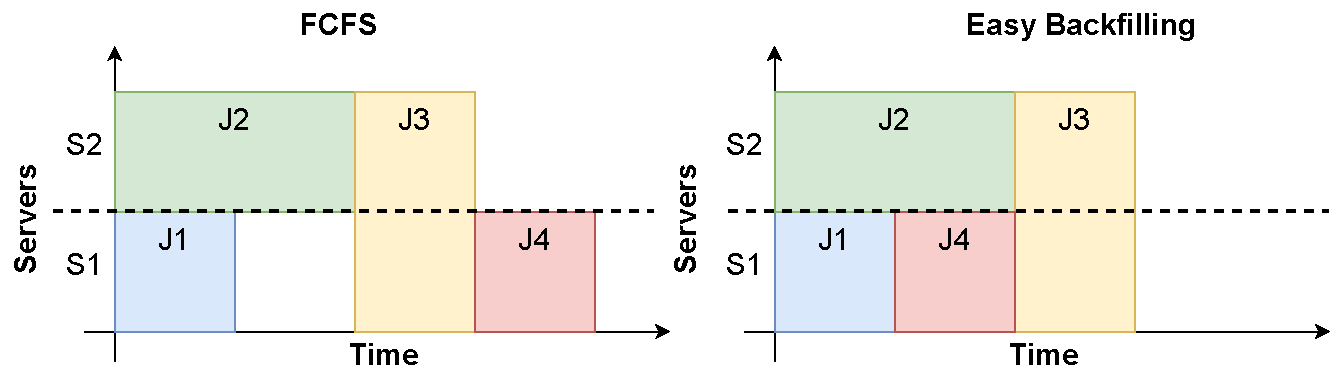
\includegraphics[scale=0.6]{Images/Related_works/backfilling.pdf}
    \caption{Comparison between FCFS and EASY Backfilling scheduling heuristics.}
    \label{fig:backfilling}
\end{figure}

Machine learning is a subfield of artificial intelligence that contains algorithms capable of automatically learning from data and improving performance on specific tasks. In some cases, they emulated the process of human learning. For example, Artificial neural networks simulate the neural network from the human brain. Another example is Reinforcement Learning (RL) which considers the trial-and-error approach, where an agent explores an environment, takes actions, and receives feedback \cite{kaelbling1996reinforcement}. Figure \ref{fig:reinforcement} illustrates this process. Through this iterative process, the agent learns to adapt its behavior by optimizing a policy. The algorithm reinforces (from where the Reinforcement Learning name comes) good actions. At some point, the algorithm stops exploring the environment and starts to use its knowledge from previous explorations to repeat what gave the best rewards. 

\begin{figure}[!htb]
    \centering
    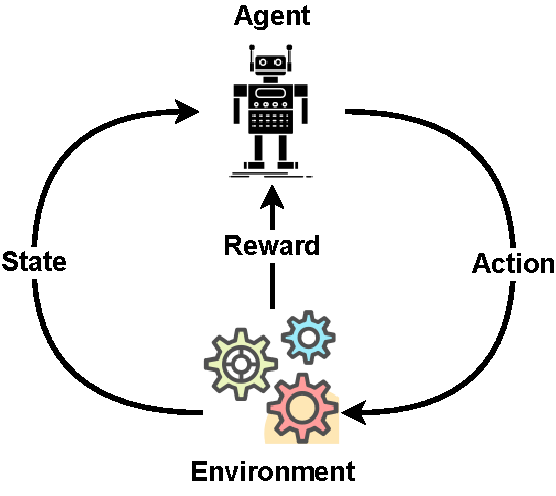
\includegraphics[scale=0.6]{Images/Related_works/Reinforcement_learning.pdf}
    \caption{Agent learning process in an environment. At each step, the agent verifies the actual state and chooses an action. The environment executes the action and returns a reward. The agent learns the reward obtained in that state for that action.}
    \label{fig:reinforcement}
\end{figure}

Finally, metaheuristics are another kind of algorithm to solve hard optimization problems. The "meta" term indicates that they are "higher level" heuristics, different from the problem-specific heuristics \cite{boussaid2013survey}. They are nature-inspired (based on some principles from physics, biology, or ethology). An example is the Genetic algorithm which simulates the evolution and mutation process from biology. Another example is Swarm algorithms inspired by the collective behavior of social insect colonies and other animal societies. Generally, metaheuristics are used to solve problems with no satisfactory problem-specific algorithm \cite{boussaid2013survey}.

In this thesis, we apply all previous methods but metaheuristics. In the offline part, we applied exact algorithms to find optimal solutions. For online, we propose heuristics to solve the specific problem. We also attempted to introduce RL to learn the environment's behavior. Since the online problem needs a fast solution for a specific problem, metaheuristics were not studied.

\section{Literature Review}
This section presents works to solve the issues related to a renewable-only data center. We verify the decisions on both offline and online levels. Some articles are not renewable only but introduce renewable in the decision process. We divided the articles into three groups: only offline, only online, and mixed decisions. The works are presented in chronological order inside each group.

\subsection{Only Offline Decisions}


\subsection{Only Online Decisions}

\citeauthor{aksanli2011utilizing} \cite{aksanli2011utilizing} presented an online heuristic that uses short-term (30 min) forecasts in the scheduling process. They implemented two queues, one for services and another for batch. Services will run independently of the green energy available, using brown if needed. Then, they predict the green energy available in the next period. Using this prediction, they estimate the number of slots available to run batch jobs. If the number is greater than the currently available slots, they schedule new jobs and spread the remainder to the running ones. If this number is smaller, the scheduler deallocates some jobs (reducing slots, killing, suspending them, or using brown energy). They compared their predictive heuristic with a reactive scheduler that allocates servers according to the energy available.

\subsection{Mixed decisions}

\subsection{Discussion and Classification of the Literature}

\begin{landscape}

\begin{table*}[htp]
\centering
\caption{Summary of characteristics for existing renewable data center scheduling works.}
\label{tab:related_works}
\begin{tabular}{m{3cm}|m{0.8cm}|m{3cm}|m{3.2cm}|m{3cm}|m{3cm}|m{3cm}}
\hline
Article & Year & Objective & Electrical infrastructure & Offline decisions & Online decisions & Method \\ \hline\hline
\citeauthor{aksanli2011utilizing} \cite{aksanli2011utilizing} & 2011 & Maximize green energy usage & Solar panels, wind turbines, and grid & - & Server and Scheduling & Heuristic \\ \hline
\citeauthor{goiri2015matching} \cite{goiri2015matching} & 2015 & Maximize green energy usage and reduce grid energy cost & Solar panels and grid & - & Server and Scheduling & Heuristic \\ \hline
\citeauthor{gu2015green} \cite{gu2015green} & 2015 & Minimize carbon emissions & Solar panels, wind turbines, and grid & Server, Scheduling, and Power & - & Exact algorithm \\ \hline
\citeauthor{li2016managing} \cite{li2016managing} & 2016 & Balance QoS, battery life span, and average backup time & Wind turbines, batteries, and grid & - & Server, Power & Heuristic \\ \hline
\citeauthor{kassab2017scheduling} \cite{kassab2017scheduling} & 2017 & Minimize makespan and flowtime & Solar panels and wind turbines & Scheduling & - & Heuristic \\ \hline
\Citeauthor{li2017balancing} \cite{li2017balancing} & 2017 & Maximize green energy usage & Solar, batteries, and grid & - & Server, Scheduling, and Power & Heuristic \\ \hline
\citeauthor{kassab2018assessing} \cite{kassab2018assessing} & 2018 & Minimize makespan and flowtime & Solar panels and wind turbines & Scheduling & - & Metaheuristic \\ \hline
\citeauthor{grange2018green} \cite{grange2018green} & 2018 & Minimize grid energy and respect QoS & Solar and grid & - & Server and Scheduling & Heuristic \\ \hline
\end{tabular}
\end{table*}

\begin{table*}[htp]
\centering
\begin{tabular}{m{3cm}|m{0.8cm}|m{3cm}|m{3.2cm}|m{3cm}|m{3cm}|m{3cm}}
\hline
Article & Year & Objective & Electrical infrastructure & Offline decisions & Online decisions & Method \\ \hline\hline
\citeauthor{hu2018schedule} \cite{hu2018schedule} & 2018 & Minimize makespan under energy constraints & - & Scheduling & - & Heuristic \\ \hline
\citeauthor{lu2018energy} \cite{lu2018energy} & 2018 & Minimize energy cost & Solar panels and grid & Scheduling and Power & - & Exact algorithm \\ \hline
\citeauthor{caux2018optimization} \cite{caux2018optimization} & 2018 & Maximize QoS under power constraints & Solar panels and wind turbines & Server and Scheduling & - & Metaheuristic and heuristic\\ \hline
\citeauthor{caux2019phase} \cite{caux2019phase} & 2019 & Maximize profit under power constraints & Solar panels and wind turbines & Server and Scheduling & - & Heuristic\\ \hline
\citeauthor{haddad2019mixed} \cite{haddad2019mixed} & 2019 & Match power demand and production & Solar panels, wind turbines, batteries, and hydrogen & Power & - & Exact algorithm \\ \hline
\citeauthor{gao2020smartly} \cite{gao2020smartly} & 2020 & Match power demand and production minimizing QoS violations & Solar panels, wind turbines, and grid & Power & - & Exact algorithm and machine learning \\ \hline
\citeauthor{haghshenas2020infrastructure} \cite{haghshenas2020infrastructure} & 2020 & Minimize energy cost & Solar panels, batteries, diesel generator, and grid & - & Scheduling, and Power & Heuristic \\ \hline
\citeauthor{nayak2021efficient} \cite{nayak2021efficient} & 2021 & Minimize makespan, energy consumption, and overall cost, and maximize renewable usage & Not specified (renewable and non-renewable without battery) & - & Scheduling & Heuristic \\ \hline
\end{tabular}
\end{table*}

\begin{table*}[htp]
\centering
\begin{tabular}{m{3cm}|m{0.8cm}|m{3cm}|m{3.2cm}|m{3cm}|m{3cm}|m{3cm}}
\hline
Article & Year & Objective & Electrical infrastructure & Offline decisions & Online decisions & Method \\ \hline\hline
\citeauthor{he2022online} \cite{he2022online} & 2021 & Minimize energy cost & Solar panels, wind turbines, and grid & - & Power & Heuristic \\ \hline
\citeauthor{peng2022energy} \cite{peng2022energy} & 2022 & Minimize energy cost & Solar panels, wind turbines, batteries, diesel generator, and grid & - & Server, Scheduling, and Power & Heuristic \\ \hline
\citeauthor{wiesner2022cucumber} \cite{wiesner2022cucumber} & 2022 & Maximize renewable excess energy usage & Solar panels and wind turbines & Scheduling & - & Heuristic \\ \hline
\citeauthor{yuan2022optimal} \cite{yuan2022optimal} & 2022 & Minimize energy cost & Solar panels, wind turbines, batteries, and grid & Power & - & Exact algorithm \\ \hline
\citeauthor{liu2023online} \cite{liu2023online} & 2023 & Minimize the energy consumption cost and carbon footprint & Grid & - & Scheduling & Machine learning \\ \hline
\citeauthor{venkataswamy2023rare} \cite{venkataswamy2023rare} & 2023 & Maximize job value (revenue) & Solar panels, wind turbines, batteries, and grid  & Server & Scheduling & Machine learning \\ \hline

\end{tabular}
\end{table*}

\end{landscape}
% \begin{itemize}
%     \item Article;
%     \item Year;
%     \item Objective;
%     \item Electrical infrastructure (solar, wind, battery, grid, etc);
%     \item Offline decisions (Scheduling, Power, Server, both);
%     \item Online decisions (Scheduling, Power, Server, both).
% \end{itemize}
% Scheduling means server on/off and job scheduling